\section{Auswertung}
\label{sec:Auswertung}
Im folgenden sind alle Amplituden in willkürlichen Einheiten angegeben.
\subsection{Vorbereitendes Experiment}
Um Redundanz zu vermeiden sind statt alle zwölf nur die Frequenzspektren, wo der Zylinder die Länge $\qty{50}{\milli\meter}$ und $\qty{600}{\milli\meter}$ hat, in der Abbildung
\ref{fig:os} aufgeführt.
\begin{figure}
\begin{subfigure}{0.48\textwidth}%
\centering%
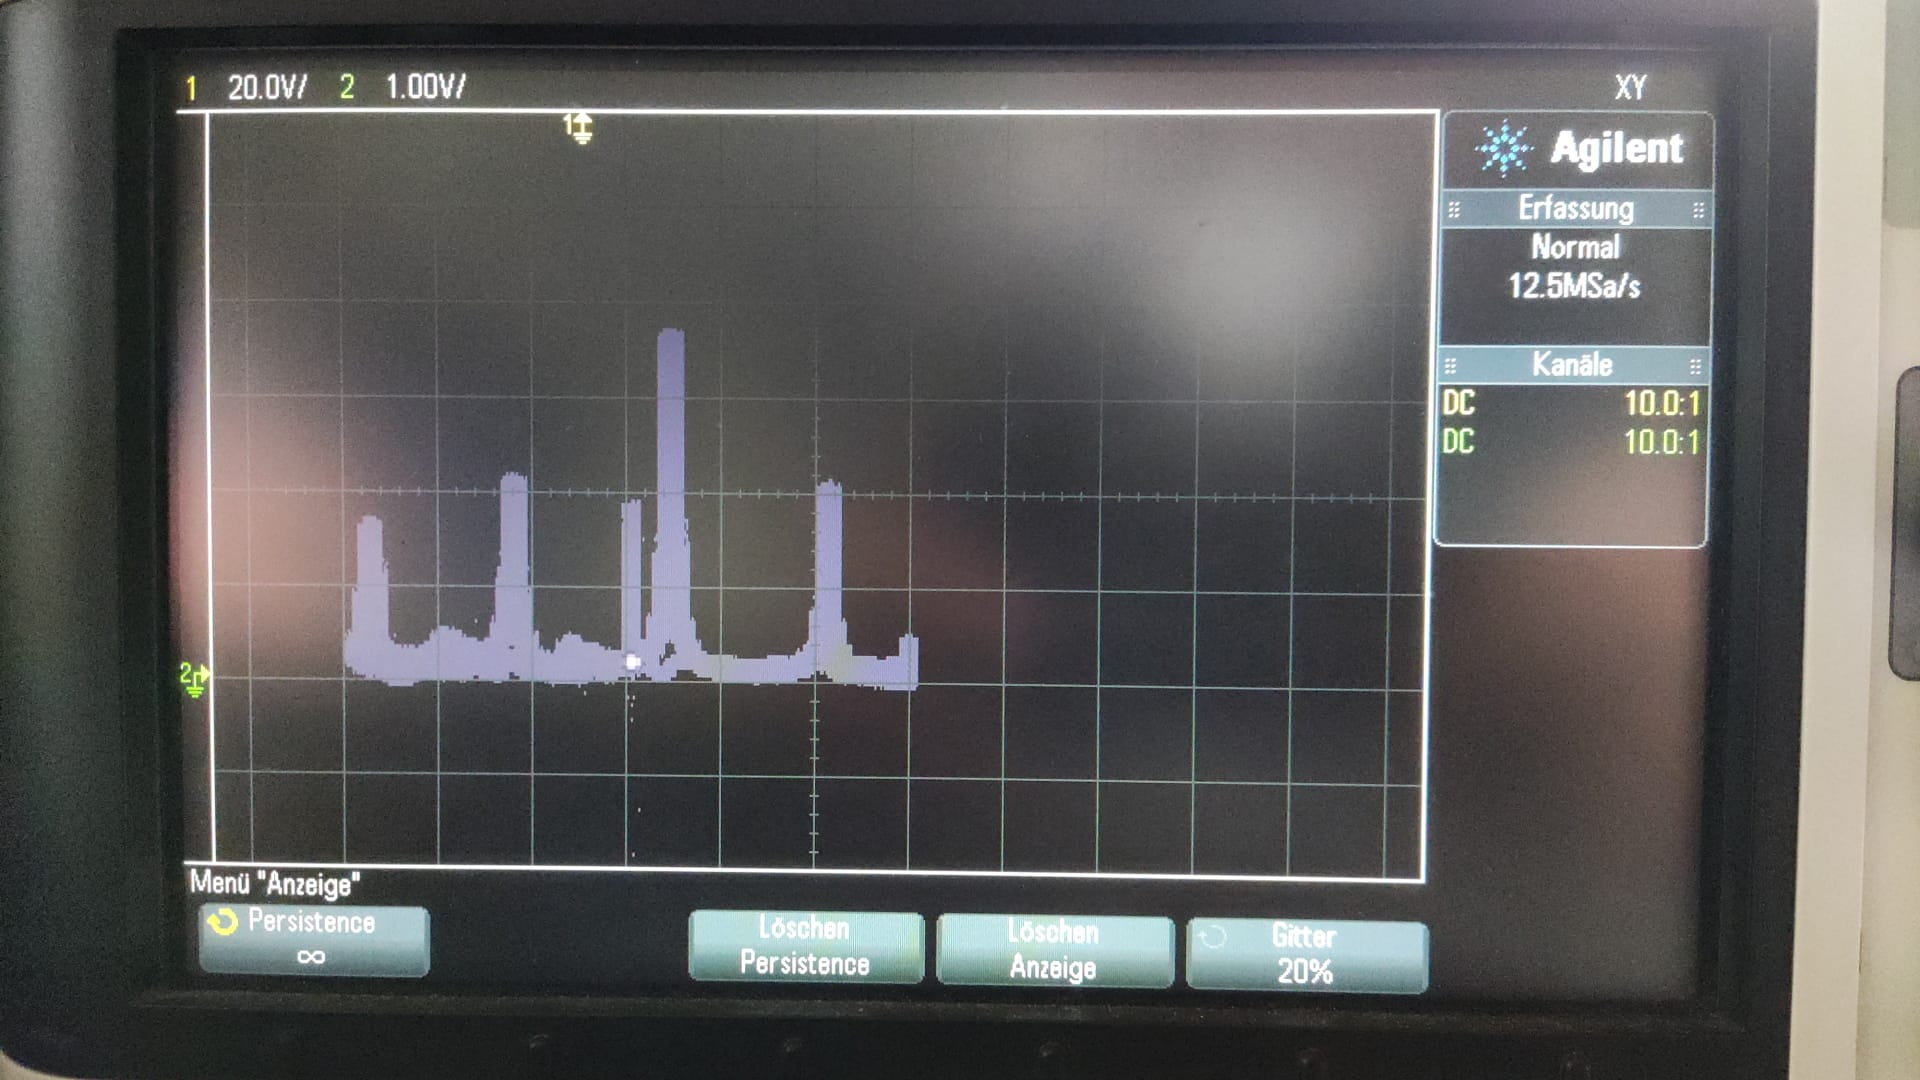
\includegraphics[height=3cm]{data_scripts/1.jpeg}%
\caption{Frequenzspektrum eines Zylinders mit der Länge $\qty{50}{\milli\meter}$}%
\label{fig:50os}%
\end{subfigure}%
\hfill% Fills available space in the center -> space between figures
\begin{subfigure}{0.48\textwidth}%
\centering%
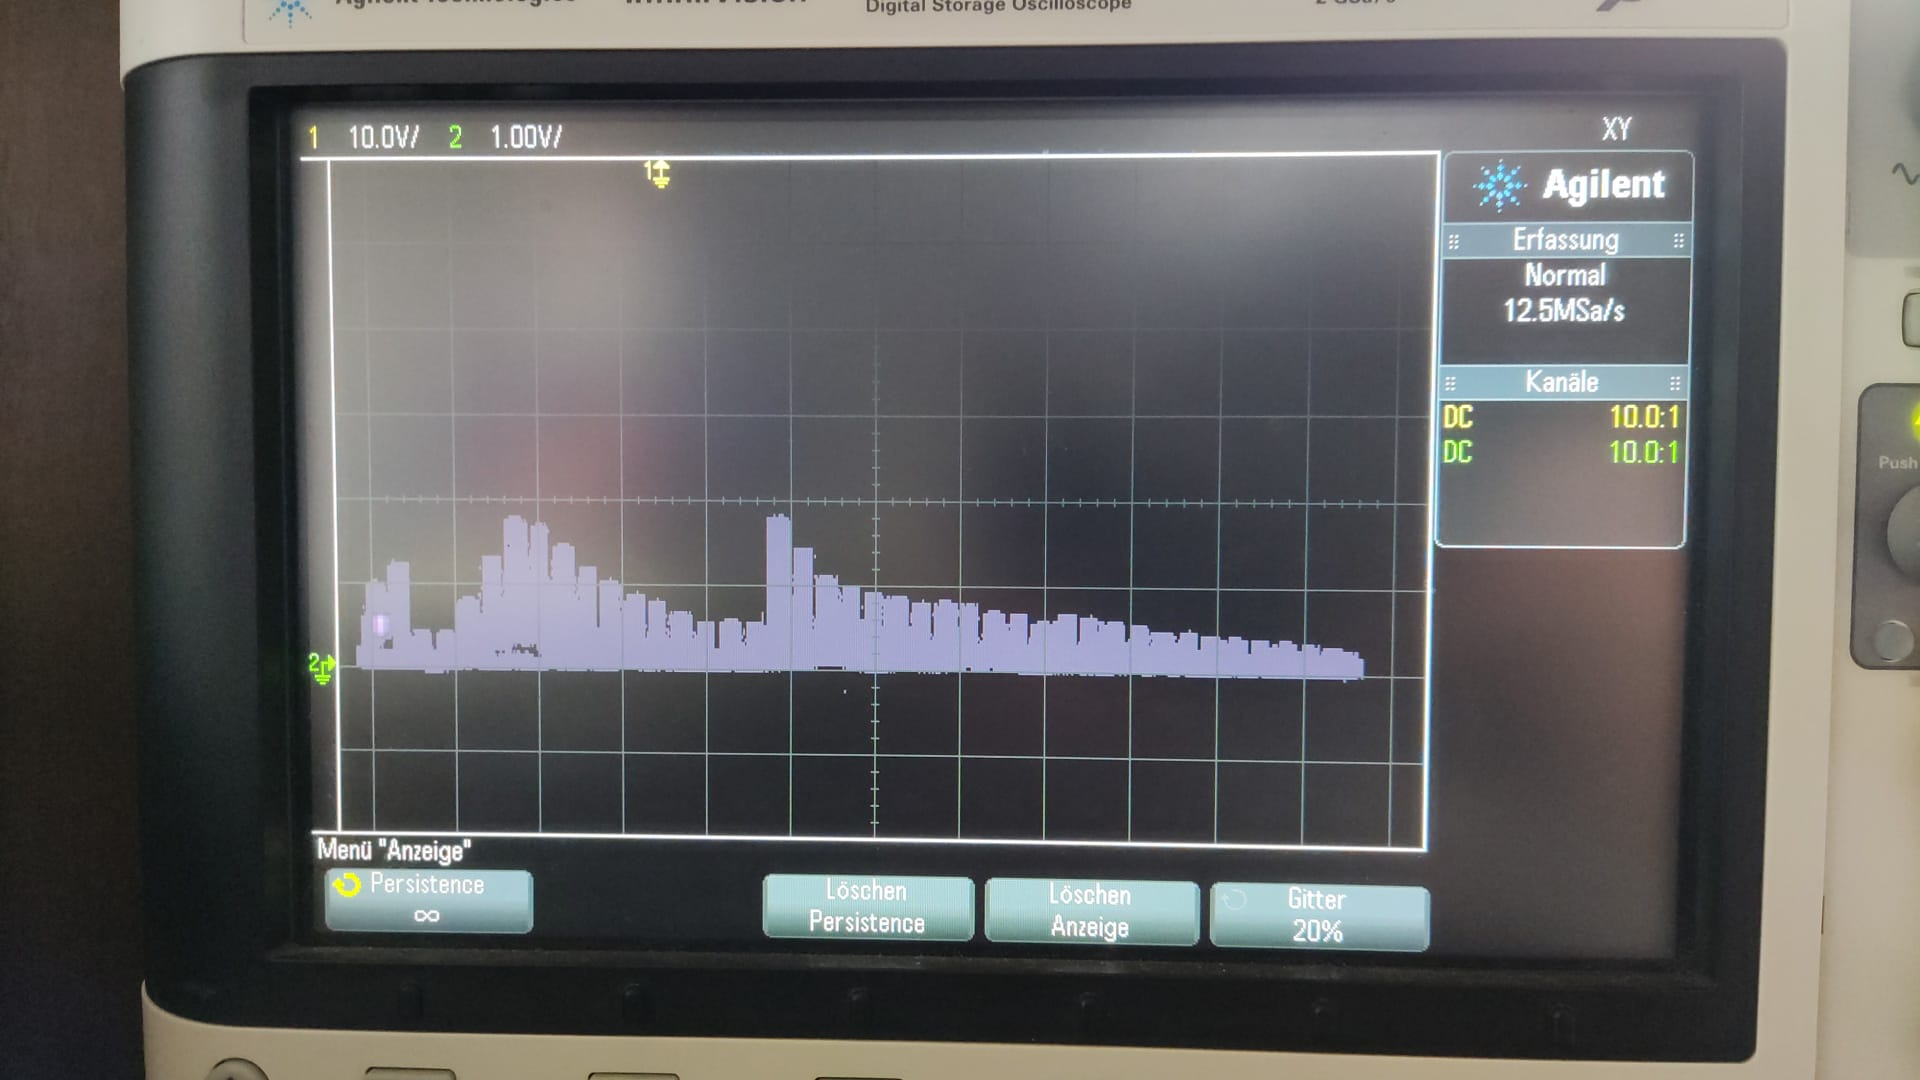
\includegraphics[height=3cm]{data_scripts/12.jpeg}%
\caption{Frequenzspektrum eines Zylinders mit der Länge $\qty{600}{\milli\meter}$}%
\label{fig:600os}%
\end{subfigure}%
\caption{Die Frequenzspektren von Zylindern mit jeweils $\qty{50}{\milli\meter}$ und $\qty{600}{\milli\meter}$, um die Frequenzspektren anderer Länge zu repräsentieren.}%
\label{fig:os}%
\end{figure}%
In der Abbildung \ref{fig:600os} wird ersichtlich, dass sich die Peaks in der Abbildung \ref{fig:50os} zu mehreren kleineren Peaks aufspalten.
Ebenfalls ist zu beobachten, dass sich der Abstand der Peaks verändert hat, denn dieser ist um ein Faktor $12$ kleiner geworden.
\subsection{Wasserstoffatom}
Um die Polarplots mit den Kugelflächenfunktionen zu vergleichen, wurden die Darstellungen der Quelle \cite{sphericalharmonics} entnommen.

\subsubsection{Hochaufgelöstes Frequenzspektrum bei sich gegenüberliegendem Mikrofon und Lautsprecher}
\begin{figure}
    \centering
    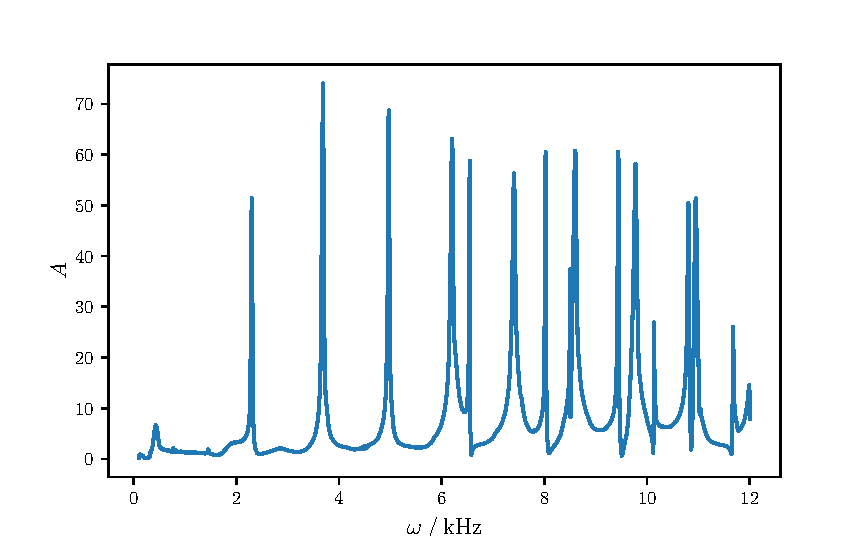
\includegraphics{build/hangle.pdf}
    \caption{Frequenzspektrum bei $\alpha = \ang{180}$}
    \label{fig:hangle}
\end{figure}
\FloatBarrier

\subsubsection{Phasenverschiebung der aufgenommenen Welle}
Die relative Phase des oberen bzw. unteren Mikrofons $\varphi_{\symup{oben}}$ und $\varphi_{\symup{unten}}$ zur Eingangswelle ist für die jeweilige Resonanzfrequenz im Intervall 
$\omega \in [\qty{100}{\hertz}\, , \qty{10}{\kilo\hertz}]$ in Tabelle 
\ref{tab:hphase} angegeben. 
Ebenfalls ist die Phasenverschiebung $\symup{\Delta}\varphi = | \varphi_{\symup{oben}} - \varphi_{\symup{unten}} |$ angegeben.
\begin{table}
    \centering
    \caption{Relative Phase zur Eingangswelle}
    \label{tab:hphase}
    \begin{tabular}{S[table-format=1.3] S[table-format=4] S[table-format=4] S[table-format=3]}
    \toprule
    {$\omega \mathbin{/} \si{\kilo\hertz}$} & $\varphi_{\symup{oben}}$ & $\varphi_{\symup{unten}}$ &{$\symup{\Delta}\varphi$} \\
    \midrule
        2.295   & 40    & 110   & 70 \\
        3.69    & -75   & 100   & 175\\
        6.24    & -40   & 33    & 73 \\
        7.43    & 0     & 180   & 180\\
        8.02    & 145   & -10   & 155\\
        8.64    & -180  & 6     & 185\\
        9.45    & -30   & -160  & 190\\
    \bottomrule
    \end{tabular}
  \end{table}
In der Tabelle \ref{tab:hphase} sind nur Phasenverschiebungen von $\approx \ang{180}$ ersichtlich.
Dies folgert, dass nur Kugelflächenfunktionen mit einer ungeraden Drehimpulsquantenzahl $l$ beobachtet wurden.
Zu den Phasenverschiebungen $\symup{\Delta}\varphi \approx \ang{70}$ lässt sich keine Aussage treffen.
\subsubsection{Amplituden in Abhängigkeit des Winkels bei Resonanzfrequenzen}
In der Abbildung \ref{fig:hvarangle27} ist die Amplitude bei der Resonanzfrequenz $\omega = \qty{2.3}{\kilo\hertz}$, in Abbildung \ref{fig:hvarangle37} bei
$\omega = \qty{3.7}{\kilo\hertz}$, in Abbildung \ref{fig:hvarangle74} bei $\omega = \qty{7.4}{\kilo\hertz}$ und in Abbildung \ref{fig:hvarangle86} bei 
$\omega = \qty{8.62}{\kilo\hertz}$ in Abhängigkeit 
des Winkels $\theta$ in einem Polarplot aufgetragen.
Der Winkel $\theta$ entspricht dabei nicht dem gemessenen Winkel $\alpha$. Zwischen den beiden Winkeln gilt die Beziehung 
\begin{equation}
    \theta = \arccos \left ( \frac{1}{2} \cos \left ( \alpha \right ) - \frac{1}{2} \right) \; {.}
\end{equation}
\begin{figure}
    \centering
    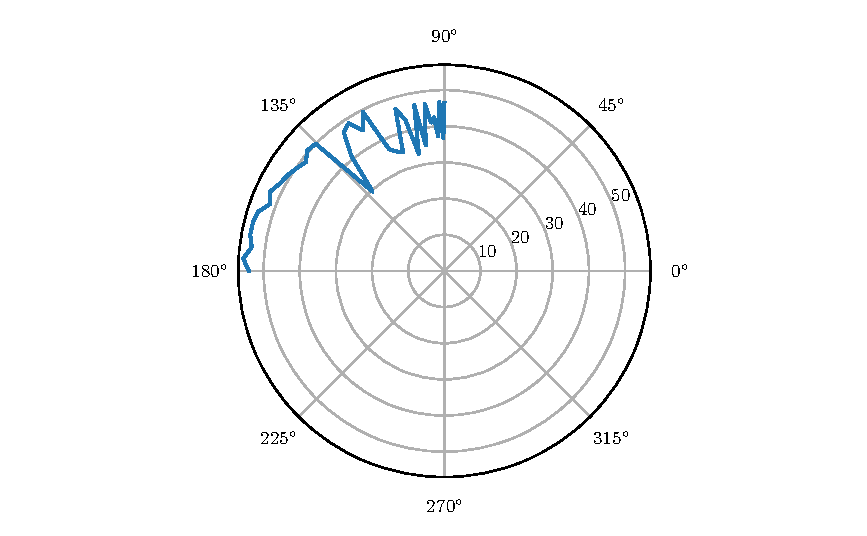
\includegraphics{build/hvarangle27.pdf}
    \caption{Polarplot des Peaks bei $\qty{2.3}{\kilo\hertz}$. Dies entspricht der Kugelflächenfunktion $Y_1^0$.}
    \label{fig:hvarangle27}
\end{figure}
\begin{figure}
    \centering
    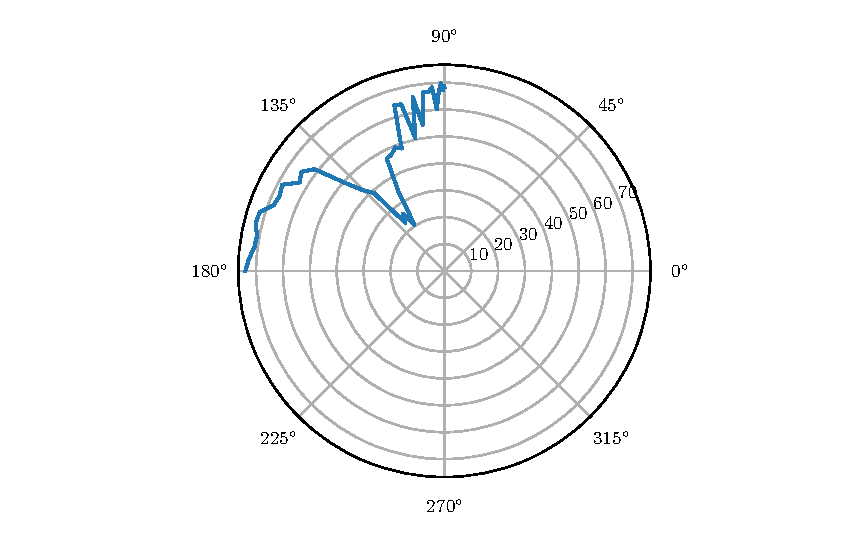
\includegraphics{build/hvarangle37.pdf}
    \caption{Polarplot des Peaks bei $\qty{3.7}{\kilo\hertz}$. Dies entspricht der Kugelflächenfunktion $Y_2^0$.}
    \label{fig:hvarangle37}
\end{figure}
\begin{figure}
    \centering
    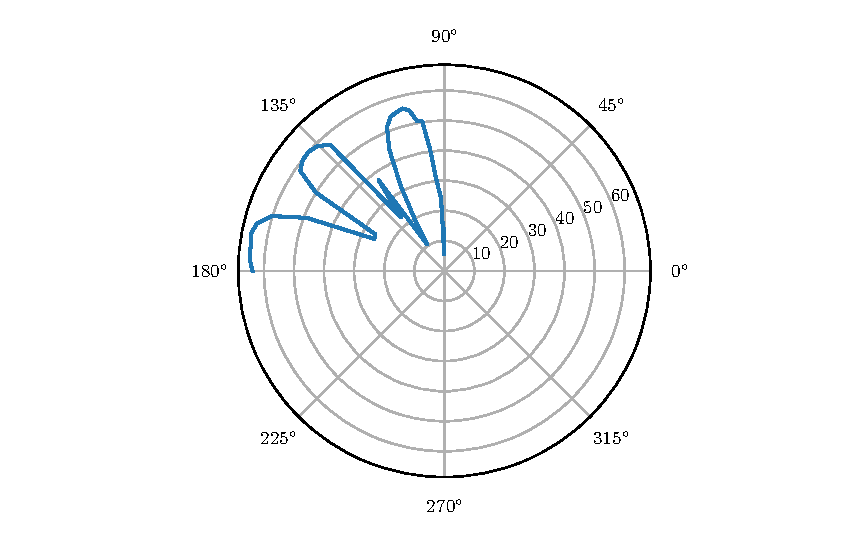
\includegraphics{build/hvarangle74.pdf}
    \caption{Polarplot des Peaks bei $\qty{7.4}{\kilo\hertz}$. Dies entspricht der Kugelflächenfunktion $Y_5^0$.}
    \label{fig:hvarangle74}
\end{figure}
\begin{figure}
    \centering
    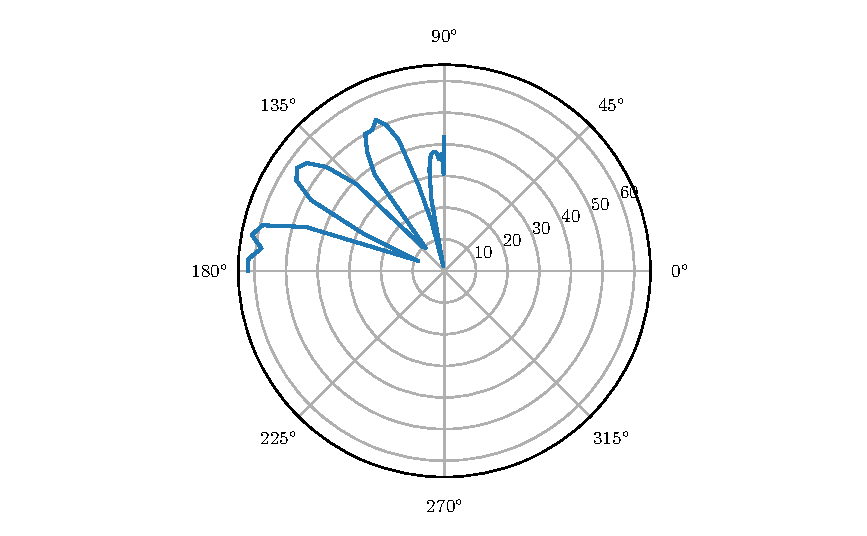
\includegraphics{build/hvarangle86.pdf}
    \caption{Polarplot des Peaks bei $\qty{8.62}{\kilo\hertz}$. Dies entspricht der Kugelflächenfunktion $Y_6^0$.}
    \label{fig:hvarangle86}
\end{figure}
\FloatBarrier

\subsubsection{Aufspaltung der Peaks bei Symmetriebrechung}
In den Abbildungen \ref{fig:h3ring2}, \ref{fig:h6ring} und \ref{fig:h9ring} sind die Frequenzspektren bei verschiedenen Ringdicken aufgezeigt.
\begin{figure}
    \centering
    \includegraphics{build/h3ring2.pdf}
    \caption{Frequenzspektrum mit einem Zwischenring der Dicke $d=\qty{3}{mm}$ bei $\alpha = \ang{180}$.}
    \label{fig:h3ring2}
\end{figure}
\begin{figure}
    \centering
    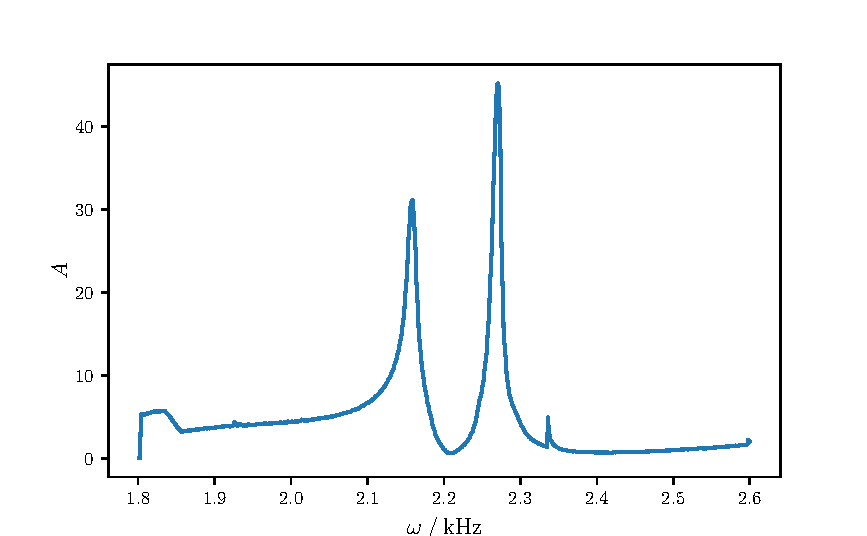
\includegraphics{build/h6ring.pdf}
    \caption{Frequenzspektrum mit einem Zwischenring der Dicke $d=\qty{6}{mm}$ bei $\alpha = \ang{180}$.}
    \label{fig:h6ring}
\end{figure}
\begin{figure}
    \centering
    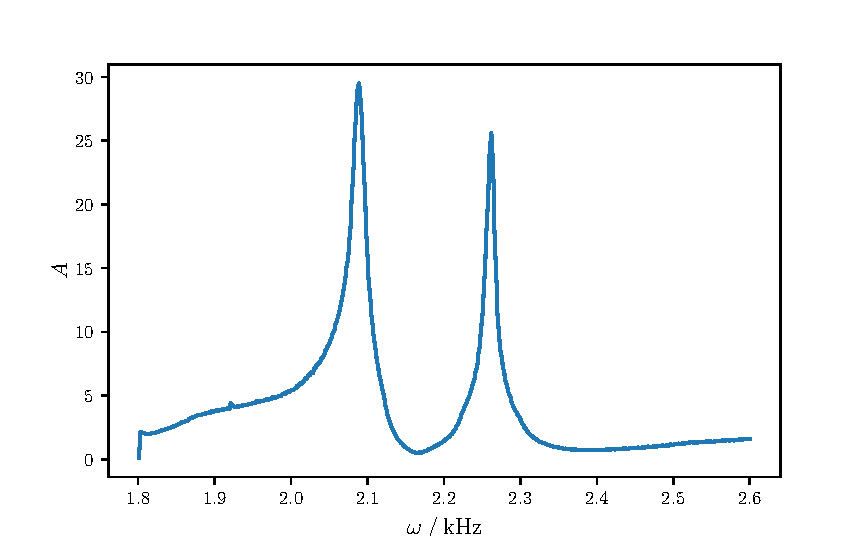
\includegraphics{build/h9ring.pdf}
    \caption{Frequenzspektrum mit einem Zwischenring der Dicke $d=\qty{9}{mm}$ bei $\alpha = \ang{180}$.}
    \label{fig:h9ring}
\end{figure}
\begin{figure}
    \centering
    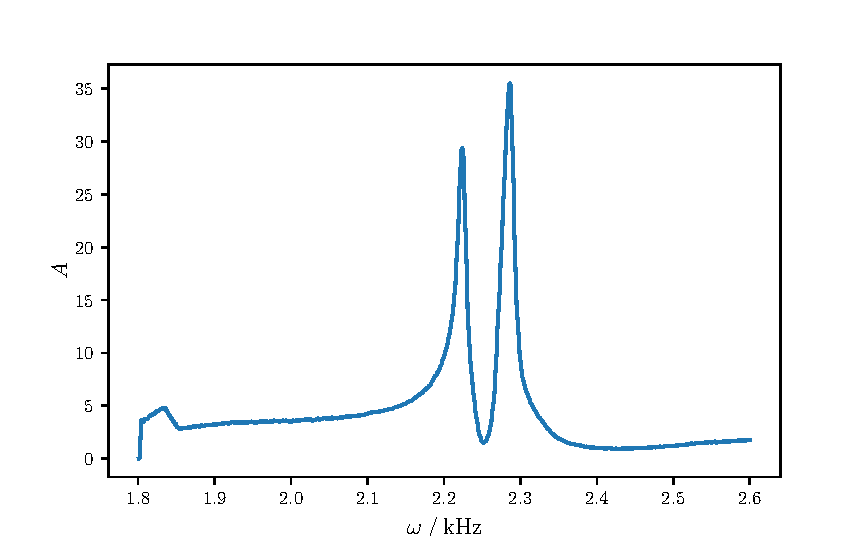
\includegraphics{build/h3ring.pdf}
    \caption{Aufspaltung der Peaks bei verschiedenen Ringdicken bei einem Winkel von $\alpha = \ang{180}$.}
    \label{fig:h3ring}
\end{figure}
Mittels Abbildung \ref{fig:h3ring} wird ersichtlich, dass die Aufspaltung der Peaks mit der Ringdicke linear zunimmt.
Dort lässt sich eine Analogie zum Zeeman-Effekt beobachten, da dort die Aufspaltung der Energien linear mit der Stärke des Magnetfelds zunimmt.
\FloatBarrier

\subsection{Wasserstoffmolekül}
\subsubsection{Abhängigkeit der Resonanzamplitude von dem Blendendurchmesser}

In den Abbildungen \ref{fig:h210} und \ref{fig:h216} sind die Frequenzspektren bei verschiedenen Blendendurchmesser aufgeführt.
\begin{figure}
    \centering
    \includegraphics{build/h210.pdf}
    \caption{Frequenzspektrum des Wasserstoffmoleküls bei einem Winkel von $\alpha = \ang{180}$ mit einer Blende mit dem Durchmesser $d = \qty{10}{\milli\meter}$.}
    \label{fig:h210}
\end{figure}

\begin{figure}
    \centering
    \includegraphics{build/h216.pdf}
    \caption{Frequenzspektrum des Wasserstoffmoleküls bei einem Winkel von $\alpha = \ang{180}$ mit einer Blende mit dem Durchmesser $d = \qty{16}{\milli\meter}$.}
    \label{fig:h216}
\end{figure}

\begin{figure}
    \centering
    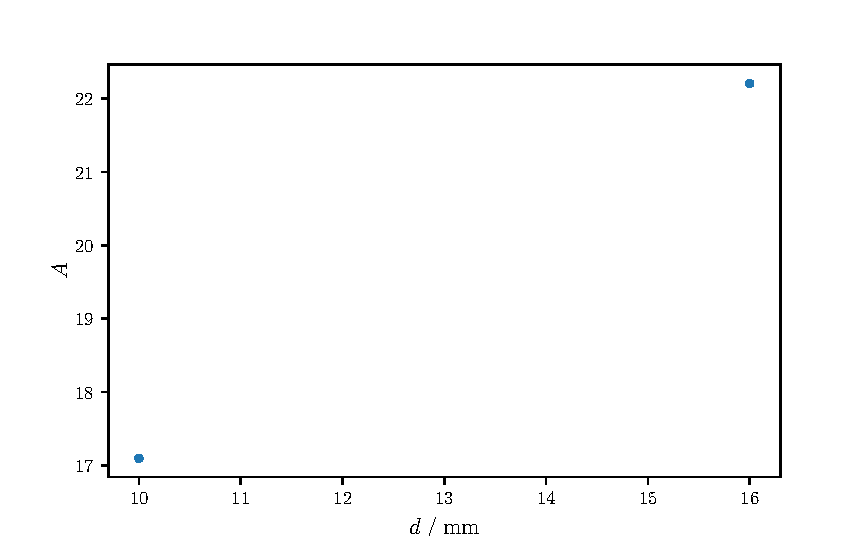
\includegraphics{build/h2dia.pdf}
    \caption{Resonanzamplitude bei $\omega = \qty{2.3}{\kilo\hertz}$ des Wasserstoffmoleküls bei einem Winkel von $\alpha = \ang{180}$ in Abhängigkeit des Blendendurchmessers.}
    \label{fig:h2dia}
\end{figure}
Anhand Abbildung \ref{fig:h2dia} lässt sich erkennen, dass ein größerer Blendendurchmesser eine größere Kopplung und somit Amplitude hervorruft.
Dies ist analog zu einem größeren Überlapp der beiden atomaren Orbitale.
\FloatBarrier

\subsubsection{Winkelabhängigkeit der Resonanzamplitude}
Der Polarplot in Abbildung \ref{fig:h2varangle}, welcher die Resonanzamplitude bei $\qty{2.3}{\kilo\hertz}$ in Abhängigkeit von dem Winkel
darstellt, bezieht auf den ersten Peak aus Abbildung \ref{fig:h2plot}.
\begin{figure}
    \centering
    \includegraphics{build/h2plot.pdf}
    \caption{Frequenzspektrum des Wasserstoffmoleküls bei einem Winkel von $\alpha = \ang{0}$.}
    \label{fig:h2plot}
\end{figure}

\begin{figure}
    \centering
    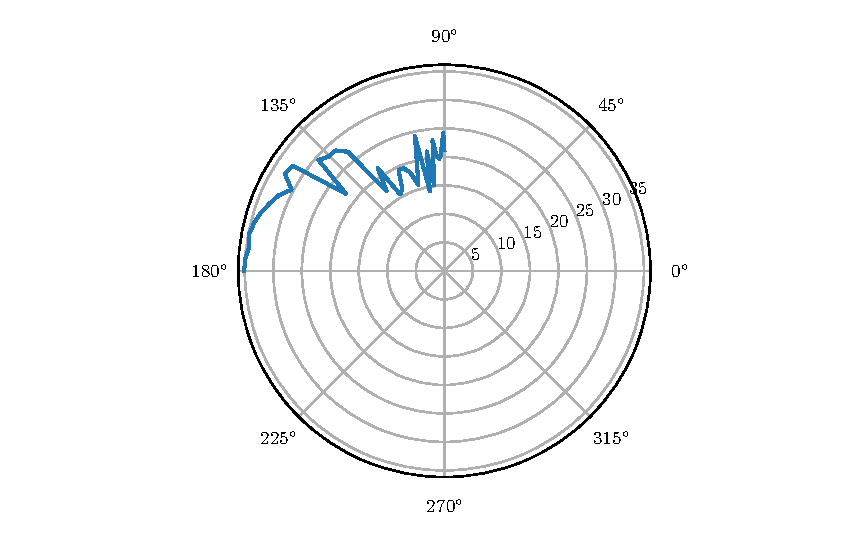
\includegraphics{build/h2varangle.pdf}
    \caption{Polarplot des Peaks bei $\qty{2.3}{\kilo\hertz}$.}
    \label{fig:h2varangle}
\end{figure}
Aufgrund der in Tabelle \ref{tab:h2phase} verschwindenen Phasenverschiebung von $\symup{\Delta}\varphi = \ang{0}$ lässt sich ein
bindender Zustand identifizieren.

\FloatBarrier
\subsubsection{Phasenverschiebung}
\begin{table}
    \centering
    \caption{Relative Phase zur Eingangswelle}
    \label{tab:h2phase}
    \begin{tabular}{S[table-format=1.3] S[table-format=4] S[table-format=4] S[table-format=3]}
    \toprule
    {$\omega \mathbin{/} \si{\kilo\hertz}$} & $\varphi_{\symup{oben}}$ & $\varphi_{\symup{unten}}$ &{$\symup{\Delta}\varphi$} \\
    \midrule
    2.295  & 0    & 0      & 0\\    
    2.48   & 7    & -172   & 179 \\
    \bottomrule
    \end{tabular}
  \end{table}
In Tabelle \ref{tab:h2phase} lässt sich erkennen, dass bei der Frequenz $\omega = \qty{2.295}{\kilo\hertz}$ ein bindender Zustand vorliegt, da die Phasenverschiebung 
$\symup{\Delta}\varphi = 0$ ist. Der Zustand bei der Frequenz $\omega = \qty{2.48}{\kilo\hertz}$ ein antibindender Zustand, da  die Phasenverschiebung 
$\symup{\Delta}\varphi = 179$ beträgt.
\FloatBarrier

\subsection{Eindimensionaler Festkörper}
\subsubsection{Festkörper aus mehreren Zylinder gleicher Länge und Blenden mit gleichem Durchmesser}
\label{subsub:dia}
\begin{figure}
    \begin{subfigure}{0.48\textwidth}%
    \centering%
    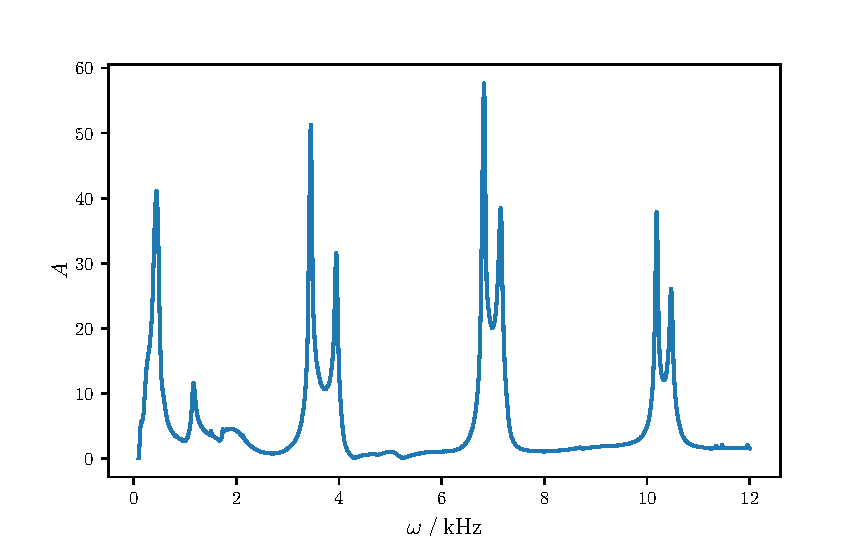
\includegraphics[height=5cm]{build/2c1b10.pdf}%
    \caption{Frequenzspektrum eines 1-dimensionalen Fesktörpers bestehend aus zwei $\qty{50}{\milli\meter}$ Zylindern und einer $\qty{10}{\milli\meter}$ Blende.}%
    \label{fig:2c1b10}%
    \end{subfigure}%
    \hfill% Fills available space in the center -> space between figures
    \begin{subfigure}{0.48\textwidth}%
    \centering%
    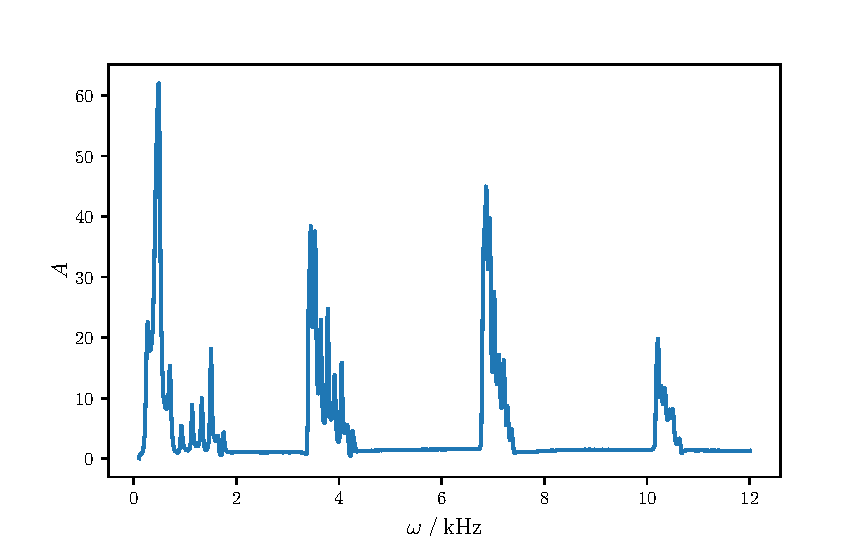
\includegraphics[height=5cm]{build/10c9b10.pdf}%
    \caption{Frequenzspektrum eines 1-dimensionalen Fesktörpers bestehend aus zehn $\qty{50}{\milli\meter}$ Zylindern und neun $\qty{10}{\milli\meter}$ Blenden.}%
    \label{fig:2c1b}%
    \end{subfigure}%
    \caption{Die Frequenzspektren von Festkörpern bestehend aus zwei bzw. zehn $\qty{50}{\milli\meter}$ Zylindern mit einer bzw. neun $\qty{10}{\milli\meter}$ Blenden, um die 
    Frequenzspektren der Festkörper, welche eine Länge zwischen diesen beiden Extrema haben, zu repräsentieren.}%
    \label{fig:10mm}
\end{figure}%
In Abbildung \ref{fig:2c1b10} wird erkenntlich, dass sich der Peak eines einzelnen Zylinders bei mehreren Zylindern und Blenden in mehrere kleinere Peaks aufspaltet.
Dies geschieht dadurch, dass die Resonanzen über mehr als einen Zylinder hinzukommen. Dies bedeutet, dass sich der Peak bei $N$ Zylindern mit einer Blende zu 
$N$ Peaks aufspaltet.
\begin{figure}
    \begin{subfigure}{0.48\textwidth}%
    \centering%
    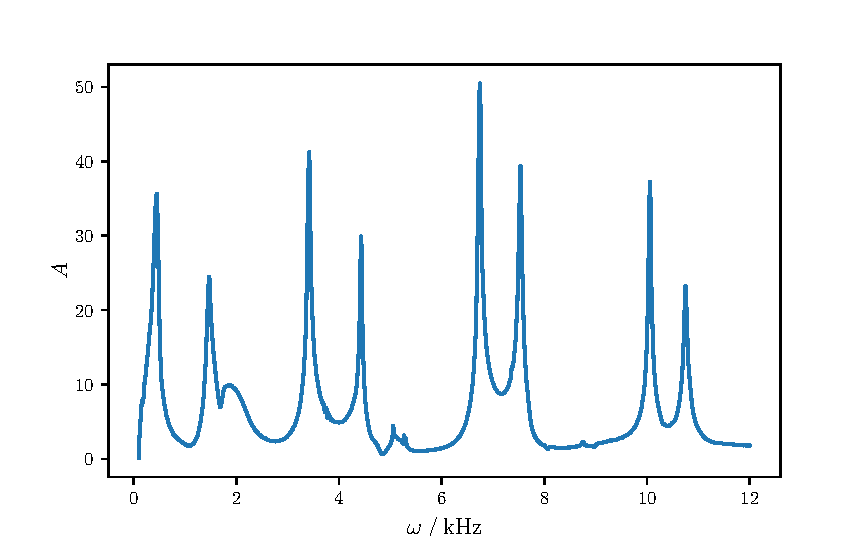
\includegraphics[height=5cm]{build/2c1b.pdf}%
    \caption{Frequenzspektrum eines 1-dimensionalen Fesktörpers bestehend aus zwei $\qty{50}{\milli\meter}$ Zylindern und einer $\qty{13}{\milli\meter}$ Blende.}%
    \label{fig:2c1b}%
    \end{subfigure}%
    \hfill% Fills available space in the center -> space between figures
    \begin{subfigure}{0.48\textwidth}%
    \centering%
    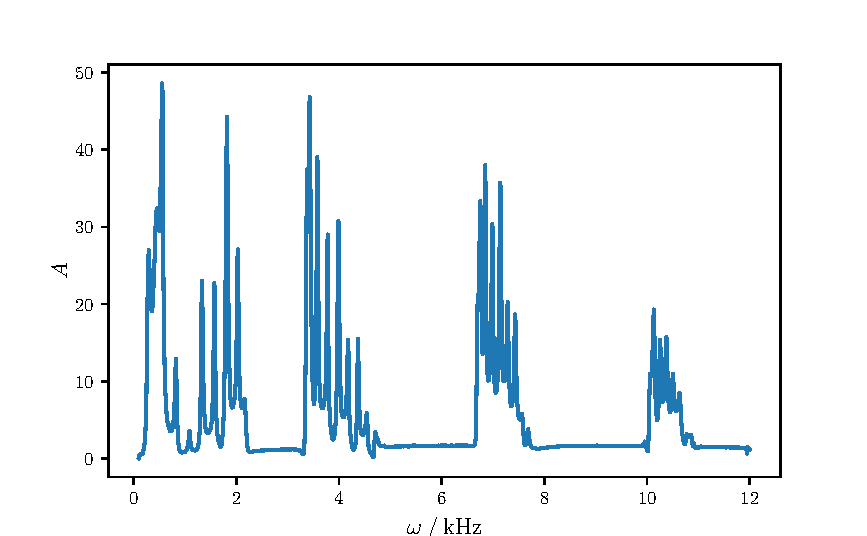
\includegraphics[height=5cm]{build/10c9b.pdf}%
    \caption{Frequenzspektrum eines 1-dimensionalen Fesktörpers bestehend aus zehn $\qty{50}{\milli\meter}$ Zylindern und neun $\qty{13}{\milli\meter}$ Blenden.}%
    \label{fig:2c1b}%
    \end{subfigure}%
    \caption{Die Frequenzspektren von Festkörpern bestehend aus zwei bzw. zehn $\qty{50}{\milli\meter}$ Zylindern mit einer bzw. neun $\qty{13}{\milli\meter}$ Blenden, um die 
    Frequenzspektren der Festkörper, welche eine Länge zwischen diesen beiden Extrema haben, zu repräsentieren.}%
    \label{fig:13mm}
\end{figure}%
Wird nun der Blendendurchmesser erhöht, verbreitern sich die Energiebänder, da die Abstände zwischen den Peaks in einem Band größer werden, 
wie in Abbildung \ref{fig:13mm} und \ref{fig:16mm} ersichtlich wird.
\FloatBarrier

\subsubsection{Ein Variabler Zylinder}
\label{subsub:varc}
In Abbildung \ref{fig:10c9b75} lässt sich ein kleiner Peak bei $\omega \approx \qty{2.2}{\kilo\hertz}$ erkennen. 
Bei den anderen Störstellen ist kein zusätzlicher Peak erkenntlich, da das Spektrum dort mit $\qty{10}{\milli\meter}$ Blenden aufgenommen wurde, und somit
die Streuung zu groß war. Ebenfalls könnte durch den kleineren Blendendurchmesser die Wechselwirkung zwischen den Rohrstücken zu klein gewesen sein, so dass dies 
auch zur Verminderung bzw. Vermeidung des zusätzlichen Peaks geführt haben.
\begin{figure}
    \begin{subfigure}{0.48\textwidth}%
    \centering%
    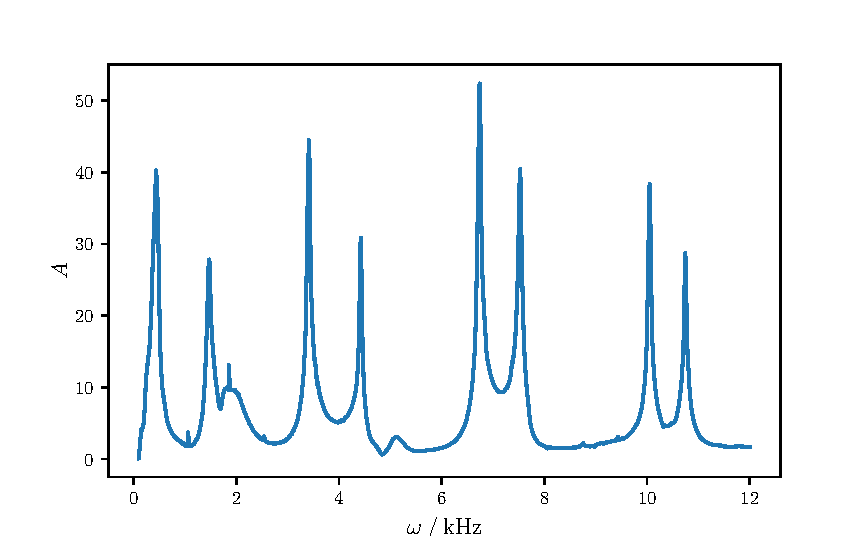
\includegraphics[height=5cm]{build/2c1b16.pdf}%
    \caption{Frequenzspektrum eines 1-dimensionalen Fesktörpers bestehend aus zwei $\qty{50}{\milli\meter}$ Zylindern und einer $\qty{16}{\milli\meter}$ Blende.}%
    \label{fig:2c1b16}%
    \end{subfigure}%
    \hfill% Fills available space in the center -> space between figures
    \begin{subfigure}{0.48\textwidth}%
    \centering%
    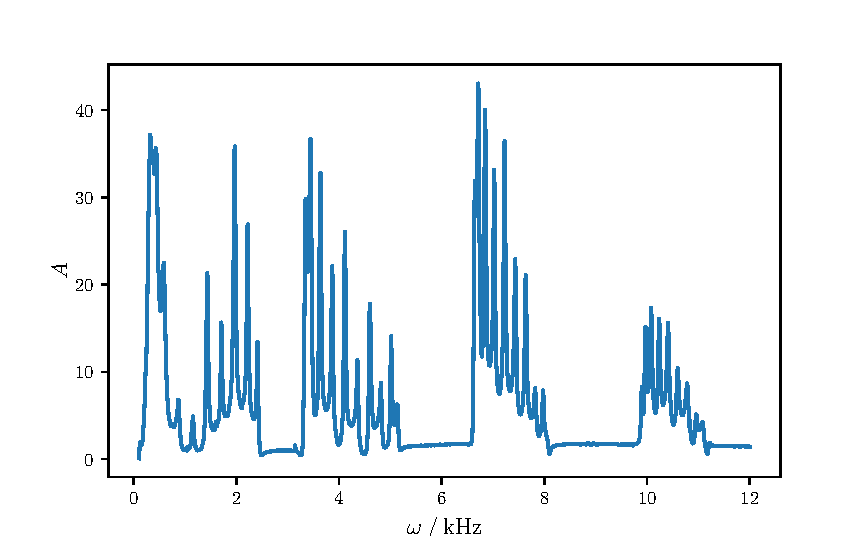
\includegraphics[height=5cm]{build/10c9b16.pdf}%
    \caption{Frequenzspektrum eines 1-dimensionalen Fesktörpers bestehend aus zehn $\qty{50}{\milli\meter}$ Zylindern und neun $\qty{16}{\milli\meter}$ Blenden.}%
    \label{fig:2c1b16}%
    \end{subfigure}%
    \caption{Die Frequenzspektren von Festkörpern bestehend aus zwei bzw. zehn $\qty{50}{\milli\meter}$ Zylindern mit einer bzw. neun $\qty{16}{\milli\meter}$ Blenden, um die 
    Frequenzspektren der Festkörper, welche eine Länge zwischen diesen beiden Extrema haben, zu repräsentieren.}%
    \label{fig:16mm}
\end{figure}%
\begin{figure}
    \begin{subfigure}{0.48\textwidth}%
        \centering%
        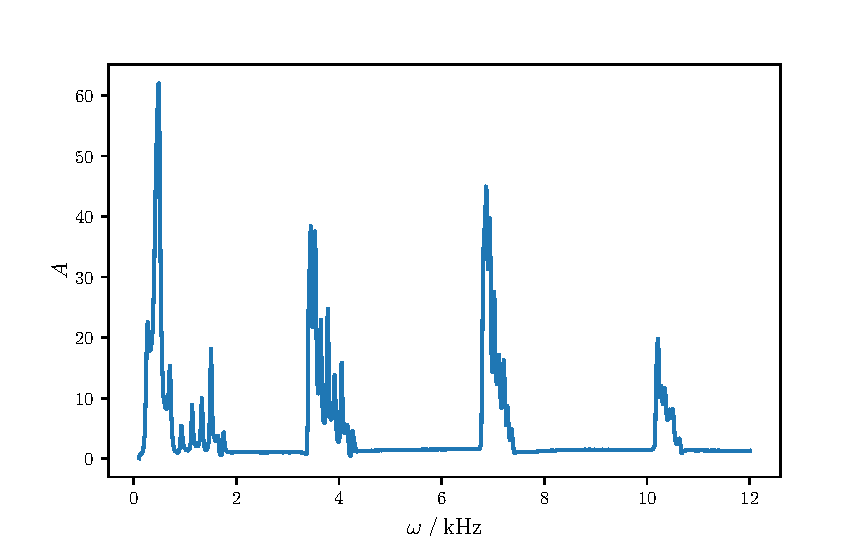
\includegraphics[height=5cm]{build/10c9b10.pdf}%
        \caption{Frequenzspektrum eines 1-dimensionalen Fesktörpers bestehend aus zehn $\qty{50}{\milli\meter}$ Zylindern und neun $\qty{10}{\milli\meter}$ Blenden.}%
        \label{fig:10c9b}%
    \end{subfigure}%
    \hfill% Fills available space in the center -> space between figures
    \begin{subfigure}{0.48\textwidth}%
        \centering%
        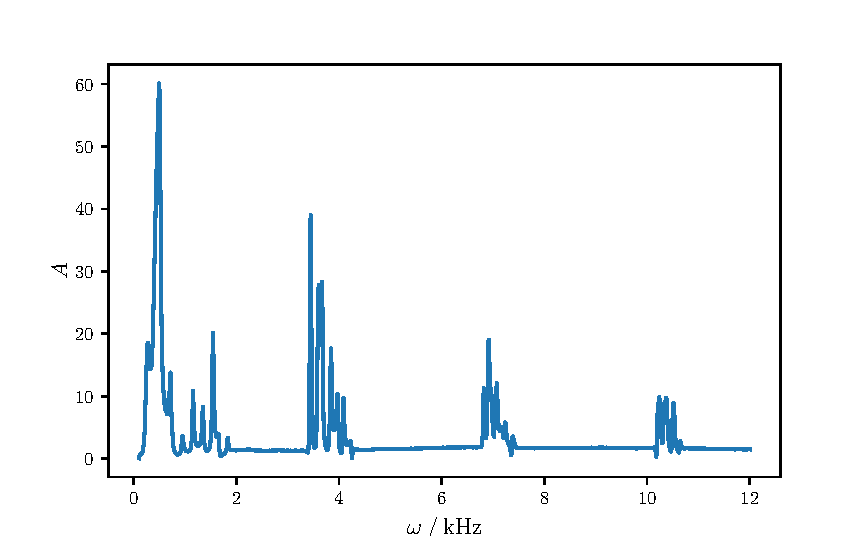
\includegraphics[height=5cm]{build/10c9b375.pdf}
        \caption{Frequenzspektrum eines 1-dimensionalen Fesktörpers bestehend aus neun $\qty{50}{\milli\meter}$ Zylindern, einem 
        $\qty{37.5}{\milli\meter}$ Zylinder und neun $\qty{10}{\milli\meter}$ Blenden.}%
        \label{fig:10c9b375}
    \end{subfigure} \\
    \begin{subfigure}{0.48\textwidth}%
        \centering%
        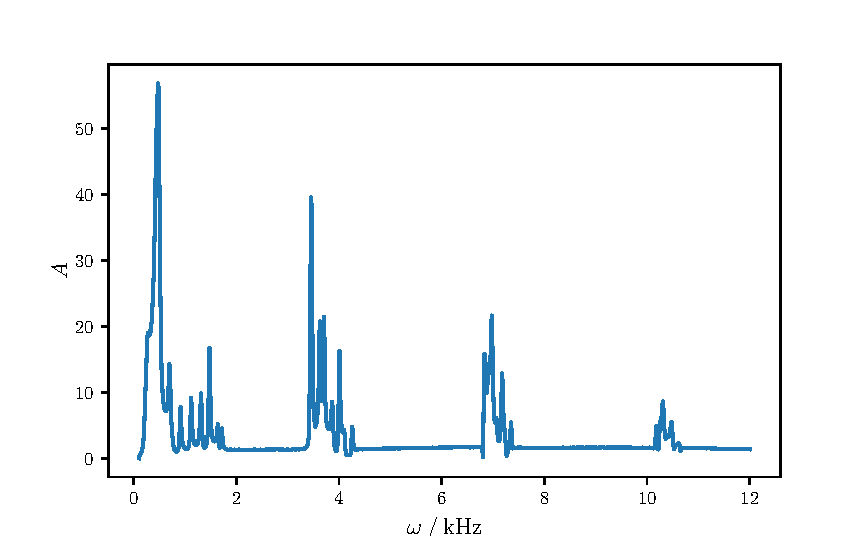
\includegraphics[height=5cm]{build/10c9b625.pdf}%
        \caption{Frequenzspektren eines 1-dimensionalen Fesktörpers bestehend aus neun $\qty{50}{\milli\meter}$ Zylindern, einem 
        $\qty{62.5}{\milli\meter}$ Zylinder und neun $\qty{10}{\milli\meter}$ Blenden.}%
        \label{fig:10c9b625}
    \end{subfigure}%
    \hfill
    \begin{subfigure}{0.48\textwidth}%
        \centering%
        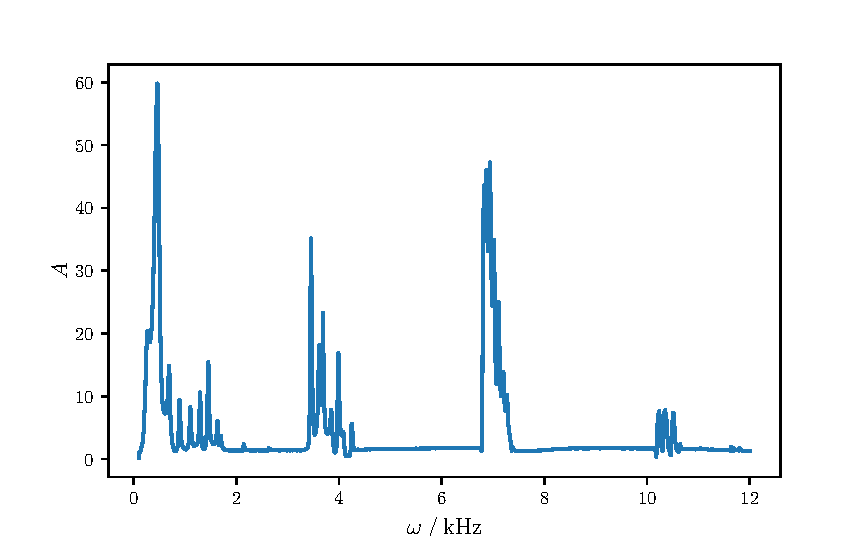
\includegraphics[height=5cm]{build/10c9b75.pdf}%
        \caption{Frequenzspektrum eines 1-dimensionalen Fesktörpers bestehend aus neun $\qty{50}{\milli\meter}$ Zylindern, einem 
        $\qty{75}{\milli\meter}$ Zylinder und neun $\qty{10}{\milli\meter}$ Blenden.}%
        \label{fig:10c9b75}
    \end{subfigure}%
    \caption{Die Frequenzspektren der Festkörper bestehend aus neun $\qty{50}{\milli\meter}$ Zylindern und einem variablen Zylinder mit neun $\qty{10}{\milli\meter}$ Blenden, um die 
            Frequenzspektren Festkörper, welche eine Länge zwischen diesen beiden Extremen haben, zu repräsentieren.}%
    \label{fig:austauschen}
\end{figure}%
\FloatBarrier

\subsection{Alternierende Zylinder und Blenden}
\label{sub:alternating}
\subsubsection{Alternierende Zylinder}
\begin{figure}
    \centering
    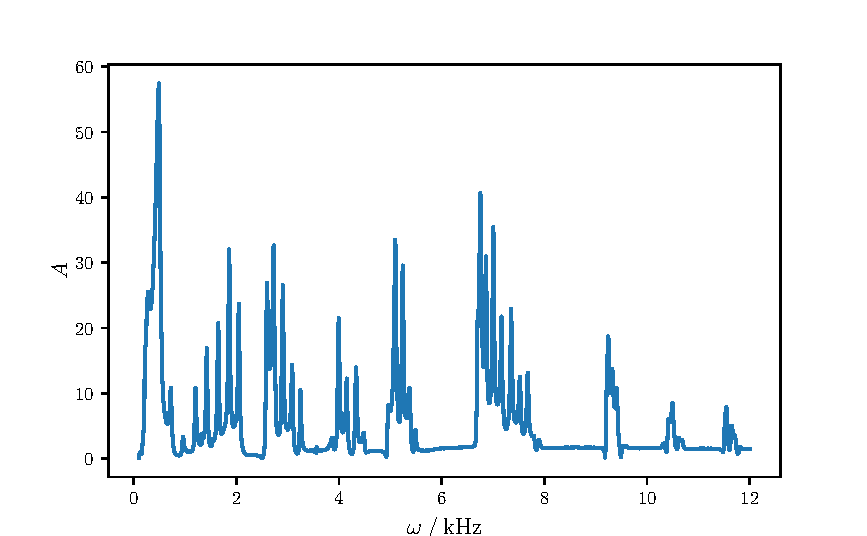
\includegraphics{build/5075.pdf}
    \caption{Frequenzspektrum eines Fesktörpers bestehend aus 10 alternierenden $\qty{50}{\milli\meter}$ und $\qty{75}{\milli\meter}$ mit neun 
    $\qty{16}{\milli\meter}$ Blenden.}
    \label{fig:5075}
\end{figure}
Beim Vergleich zu Abbildung \ref{fig:75and50single} fallen die Peaks in Abbildung \ref{fig:5075}, welche den Peaks von den einzelnen Rohren mit einem Durchmesser von 
$d = \qty{50}{\milli\meter}$ bzw. $d = \qty{75}{\milli\meter}$ entsprechen, auf. 
\begin{figure}
    \begin{subfigure}{0.48\textwidth}%
        \centering%
        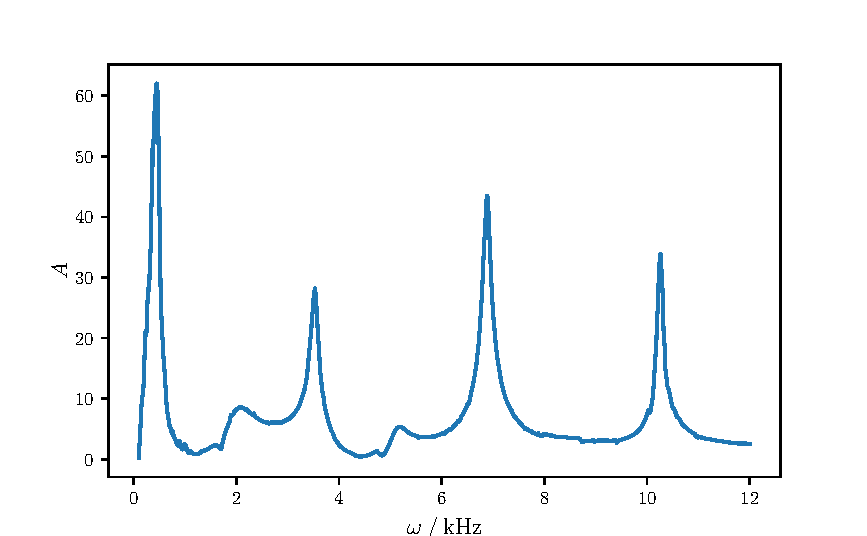
\includegraphics[height=5cm]{build/50single.pdf}%
        \caption{Frequenzspektrum von einem einzelnen $\qty{50}{\milli\meter}$ Zylinder.}%
        \label{fig:50sinlge}%
    \end{subfigure}%
    \hfill% Fills available space in the center -> space between figures
    \begin{subfigure}{0.48\textwidth}%
        \centering%
        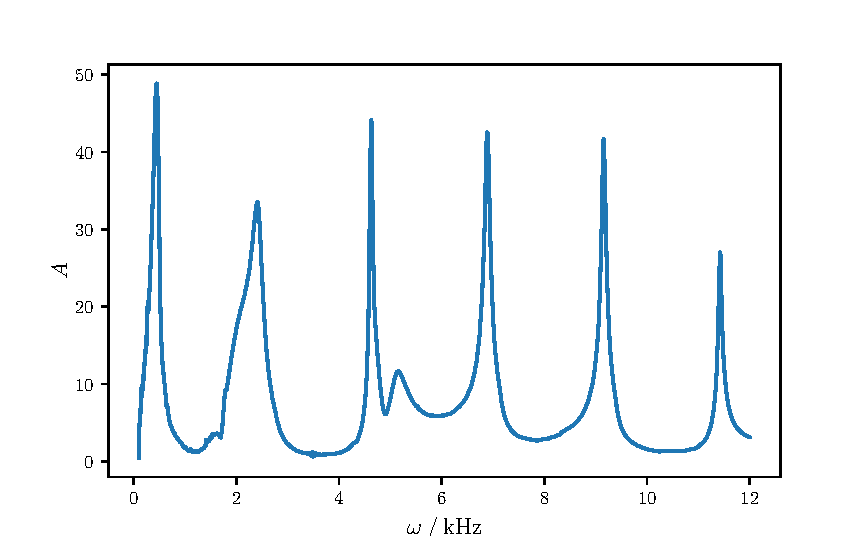
\includegraphics[height=5cm]{build/75single.pdf}%
        \caption{Frequenzspektrum von einem einzelnen $\qty{75}{\milli\meter}$ Zylinder.}%
        \label{fig:75single}%
    \end{subfigure}%
    \caption{Die Frequenzspektren von einzelnen $\qty{50}{\milli\meter}$ bzw. $\qty{75}{\milli\meter}$ Zylindern, um diese mit dem Spektrum
    aus Abbildung \ref{fig:5075} zu vergleichen.}%
    \label{fig:75and50single}
\end{figure}%
\FloatBarrier

\subsubsection{Alternierende Blendendurchmesser}
Wenn nun die Blenden alternierend angeordnet werden, gleicht dies einem Festkörper bestehend aus zwei Basisatomen, wodurch zwei Untergitter simuliert werden.
In Abbildung \ref{fig:1316} wird deutlich, dass die Periodizität der verschiedenen Zylinderlängen ein Analogon zu zwei Untergittern ist. 
\begin{figure}
    \centering
    \includegraphics{build/1316.pdf}
    \caption{Frequenzspektrum eines Festkörpers bestehend aus acht $\qty{50}{\milli\meter}$ Zylindern mit sieben alternierenden einzelnen $\qty{13}{\milli\meter}$ und 
    $\qty{16}{\milli\meter}$ Blenden.}
    \label{fig:1316}
\end{figure}
Bei alternierenden Blendendurchmesser entstehen neben den Hauptbündeln an Peaks neue Nebenbündel an Peaks, was mit der Beobachtung aus \ref{subsub:dia} übereinstimmt.
Diese neuen Nebenbündel entsprechen neuen Subbändern.